\tikzset{every picture/.style={line width=0.75pt}} %set default line width to 0.75pt        
\noindent
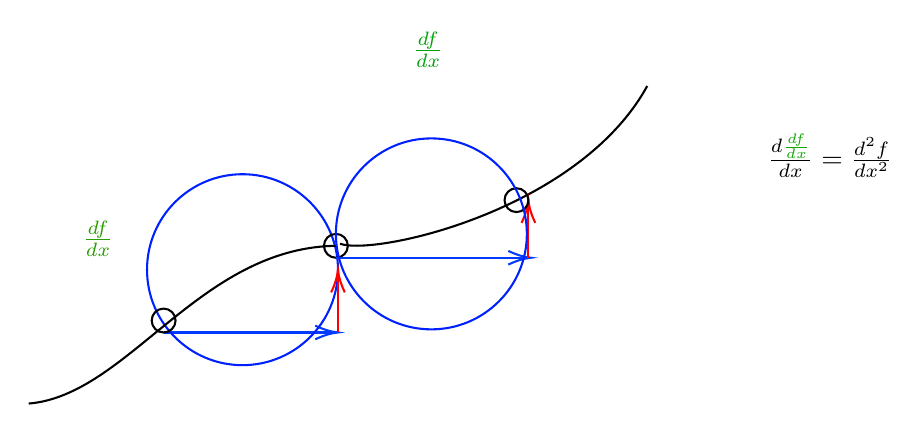
\begin{tikzpicture}[x=0.75pt,y=0.75pt,yscale=-1,xscale=1]
%uncomment if require: \path (0,300); %set diagram left start at 0, and has height of 300

%Straight Lines [id:da5249154936080698] 
\draw [color={rgb, 255:red, 0; green, 59; blue, 255 }  ,draw opacity=1 ]   (166.5,177.75) -- (248.5,177.75) ;
\draw [shift={(250.5,177.75)}, rotate = 180] [color={rgb, 255:red, 0; green, 59; blue, 255 }  ,draw opacity=1 ][line width=0.75]    (10.93,-3.29) .. controls (6.95,-1.4) and (3.31,-0.3) .. (0,0) .. controls (3.31,0.3) and (6.95,1.4) .. (10.93,3.29)   ;
%Shape: Circle [id:dp6264518317388023] 
\draw  [color={rgb, 255:red, 0; green, 33; blue, 255 }  ,draw opacity=1 ] (158.5,147.5) .. controls (158.5,122.09) and (179.09,101.5) .. (204.5,101.5) .. controls (229.91,101.5) and (250.5,122.09) .. (250.5,147.5) .. controls (250.5,172.91) and (229.91,193.5) .. (204.5,193.5) .. controls (179.09,193.5) and (158.5,172.91) .. (158.5,147.5) -- cycle ;
%Curve Lines [id:da7807839624552354] 
\draw    (101.5,212) .. controls (149.5,208) and (183.5,137) .. (249.5,136) ;
%Straight Lines [id:da9914689490458466] 
\draw [color={rgb, 255:red, 255; green, 0; blue, 0 }  ,draw opacity=1 ]   (250.5,177.75) -- (250.5,149.5) ;
\draw [shift={(250.5,147.5)}, rotate = 450] [color={rgb, 255:red, 255; green, 0; blue, 0 }  ,draw opacity=1 ][line width=0.75]    (10.93,-3.29) .. controls (6.95,-1.4) and (3.31,-0.3) .. (0,0) .. controls (3.31,0.3) and (6.95,1.4) .. (10.93,3.29)   ;
%Shape: Circle [id:dp6225217552848006] 
\draw   (160.75,172) .. controls (160.75,168.82) and (163.32,166.25) .. (166.5,166.25) .. controls (169.68,166.25) and (172.25,168.82) .. (172.25,172) .. controls (172.25,175.18) and (169.68,177.75) .. (166.5,177.75) .. controls (163.32,177.75) and (160.75,175.18) .. (160.75,172) -- cycle ;
%Shape: Circle [id:dp7604395975548914] 
\draw   (243.75,136) .. controls (243.75,132.82) and (246.32,130.25) .. (249.5,130.25) .. controls (252.68,130.25) and (255.25,132.82) .. (255.25,136) .. controls (255.25,139.18) and (252.68,141.75) .. (249.5,141.75) .. controls (246.32,141.75) and (243.75,139.18) .. (243.75,136) -- cycle ;
%Straight Lines [id:da09696007717899835] 
\draw [color={rgb, 255:red, 0; green, 59; blue, 255 }  ,draw opacity=1 ]   (249.5,141.75) -- (341.5,141.75) ;
\draw [shift={(343.5,141.75)}, rotate = 180] [color={rgb, 255:red, 0; green, 59; blue, 255 }  ,draw opacity=1 ][line width=0.75]    (10.93,-3.29) .. controls (6.95,-1.4) and (3.31,-0.3) .. (0,0) .. controls (3.31,0.3) and (6.95,1.4) .. (10.93,3.29)   ;
%Curve Lines [id:da7296977853270968] 
\draw    (251.5,135) .. controls (268.5,141) and (366.5,119) .. (399.5,59) ;
%Straight Lines [id:da7467496809128916] 
\draw [color={rgb, 255:red, 255; green, 0; blue, 0 }  ,draw opacity=1 ]   (342.25,141.75) -- (342.25,116) ;
\draw [shift={(342.25,114)}, rotate = 450] [color={rgb, 255:red, 255; green, 0; blue, 0 }  ,draw opacity=1 ][line width=0.75]    (10.93,-3.29) .. controls (6.95,-1.4) and (3.31,-0.3) .. (0,0) .. controls (3.31,0.3) and (6.95,1.4) .. (10.93,3.29)   ;
%Shape: Circle [id:dp3804669744025936] 
\draw   (330.75,114) .. controls (330.75,110.82) and (333.32,108.25) .. (336.5,108.25) .. controls (339.68,108.25) and (342.25,110.82) .. (342.25,114) .. controls (342.25,117.18) and (339.68,119.75) .. (336.5,119.75) .. controls (333.32,119.75) and (330.75,117.18) .. (330.75,114) -- cycle ;
%Shape: Circle [id:dp8826731960000049] 
\draw  [color={rgb, 255:red, 0; green, 33; blue, 255 }  ,draw opacity=1 ] (249.5,130.25) .. controls (249.5,104.84) and (270.09,84.25) .. (295.5,84.25) .. controls (320.91,84.25) and (341.5,104.84) .. (341.5,130.25) .. controls (341.5,155.66) and (320.91,176.25) .. (295.5,176.25) .. controls (270.09,176.25) and (249.5,155.66) .. (249.5,130.25) -- cycle ;

% Text Node
\draw (126,122.4) node [anchor=north west][inner sep=0.75pt]  [color={rgb, 255:red, 40; green, 158; blue, 0 }  ,opacity=1 ]  {$\frac{df}{dx}$};
% Text Node
\draw (285,31.4) node [anchor=north west][inner sep=0.75pt]  [color={rgb, 255:red, 1; green, 163; blue, 10 }  ,opacity=1 ]  {$\frac{df}{dx}$};
% Text Node
\draw (456,80.4) node [anchor=north west][inner sep=0.75pt]    {$\frac{d\textcolor[rgb]{0.07,0.65,0.01}{\frac{df}{dx}}}{dx} =\frac{d^{2} f}{dx^{2}}$};


\end{tikzpicture}
